\subsection{Marketing}
È la funzione d'impresa che identifica i \textbf{BISOGNI}, i \textbf{COMPORTAMENTI}, le \textbf{ASPETTATIVE} ed i \textbf{DESIDERI} (espressi e inespressi) insoddisfatti, che ne definisce l'ampiezza, che determina quali mercati obiettivo l'impresa può meglio servire, che definisce il valore da offrire attraverso prodotti/servizi e i programmi rivolti ai mercati suddetti, che sollecita tutte le componenti dell'azienda a pensare in termini di servizio al cliente e gestione della relazione.

Il \textit{marketing} è l'interfaccia tra azienda e cliente.

\subsubsection{Marketing Strategico}
Analizza i bisogni dei clienti e definisce il mercato di riferimento dell’impresa (orizzonte di riferimento di medio lungo periodo). A causa dell’eterogeneità dei bisogni della clientela, essa deve essere suddivisa o segmentata in gruppi omogenei al loro interno ed eterogenei fra loro.

Il \textit{marketing} strategico è una programmazione di ampio respiro, che può durare pochi mesi o diversi anni, e che ha come obiettivo principale studiare il mercato al fine di ottimizzare gli strumenti di comunicazione e raggiungere obiettivi di maggior guadagno con minor sforzo e in minor tempo.
Ha l’arduo e stimolante compito di portare un concreto vantaggio competitivo all’azienda grazie ad un’attenta pianificazione delle attività di \textit{marketing} e comunicazione.

Attraverso una visione del mercato e dei suoi mutamenti il più possibile completa, un’analisi attenta delle opportunità e dei rischi, è possibile infatti sviluppare una filosofia aziendale orientata al cliente che sia in grado di creare valore tangibile per l’azienda.

La segmentazione del mercato è il processo mediante il quale si suddivide il mercato in un numero limitato di segmenti, ognuno dei quali sufficientemente omogeneo per motivazioni, comportamenti e scelte, ma nello stesso tempo abbastanza differenziato dagli altri.
La scelta fondamentale che caratterizza la strategia di marketing è relativa alla definizione dei mercati di riferimento:
\begin{itemize}
	\item \textit{Marketing} di massa o indifferenziato 
	\item \textit{Marketing} differenziato
	\item \textit{Marketing} concentrato
\end{itemize}
Per la costruzione di tale spazio, si devono identificare i seguenti punti:
\begin{enumerate}[label=\alph*)]
	\item L’identificazione di un insieme di dimensioni che rappresentino gli attributi salienti per i quali i consumatori scelgono un dato prodotto
	\item Una scala di misurazione del valore assegnato
	\item La rappresentazione grafica di questi valori su più dimensioni
\end{enumerate}
Il posizionamento definisce il modo in cui l’impresa e/o il prodotto sono percepiti dagli acquirenti potenziali, in relazione ai concorrenti. Per definire il posizionamento in maniera operativa le imprese individuano uno spazio multidimensionale dove ciascun prodotto o marca occupa una determinata posizione.
I problemi che il marketing strategico risolve sono:
\begin{itemize}
	\item Il piano \textit{marketing} parte dalla definizione di obiettivi organizzativi che siano misurabili e soprattutto chiari, che permettano di fare le giuste scelte di pianificazione.
	\item In prima battuta quindi il marketing strategico permette di fare il punto della situazione e stabilire obiettivi razionali attraverso la determinazione delle aree di \textit{business}.
	\item Grazie ad un piano \textit{marketing} inoltre è possibile individuare nuove opportunità in diversi segmenti di mercato o nel ciclo di vita del prodotto o bisogni ancora non ben individuati nel nostro \textit{target}.
	\item Il piano \textit{marketing} inoltre aiuta a semplificare le strategie adottabili, razionalizzarle e indicare il giusto percorso attraverso la definizione di azioni precise. In poche parole permette di fare ordine nel caos teorico, anche mutando più volte nel corso del tempo, adattandosi al contesto sempre mutevole e strutturando un piano operativo definito e attuabile nei tempi e nei modi giusti.
\end{itemize}

\begin{figure}[h]
	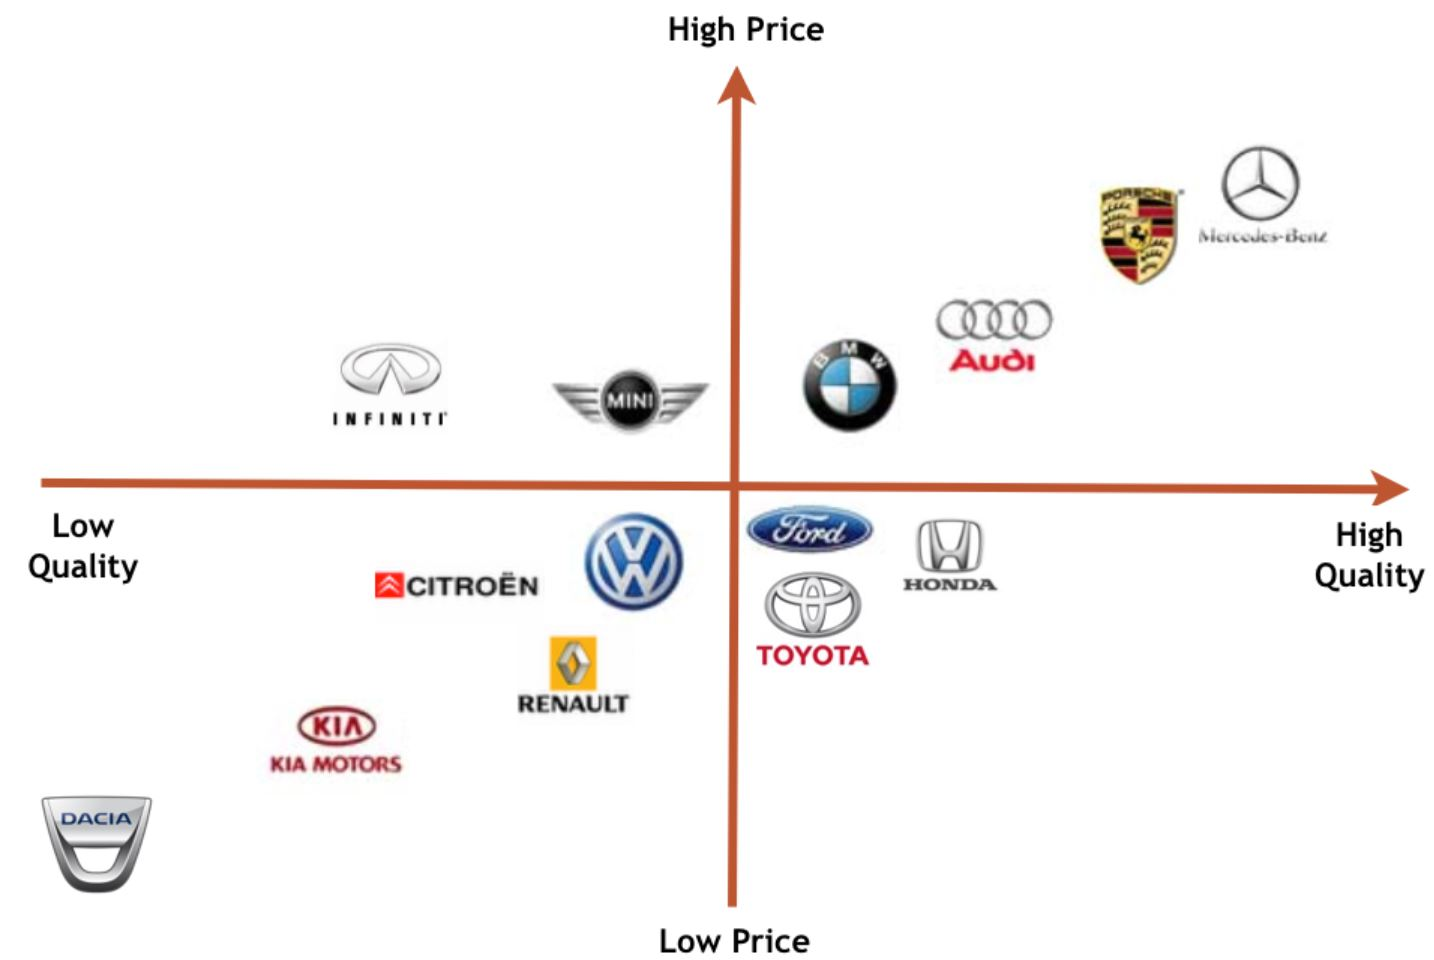
\includegraphics[width=0.6\linewidth]{resources/chapters/OrganizzazioneAziendale/images/mappa-posizionamento.jpg}
	\centering
	\caption{Mappa che raffigura il posizionamento di mercato nel settore automobilistico}
\end{figure}

Il \textit{marketing} strategico si può riassumere in:
\begin{itemize}
	\item Ricerca ed elabora le opportunità di mercato
	\item Definisce i segmenti di mercato
	\item Identifica le aspettative del cliente
\end{itemize}

\newpage
\subsubsection{Marketing Operativo}
Il \textit{marketing} operativo è la parte finale dell’intero processo di \textit{marketing}, a monte del quale ci sono le fasi di marketing analitico e marketing strategico. Solo dopo aver studiato i dati dell’azienda e dei concorrenti e aver pianificato le operazioni da eseguire, arriva il momento dell’azione. La componente operativa (o tattica) del \textit{marketing} ha il compito di realizzare concretamente le strategie definite nelle fasi precedenti, disponendo delle risorse (denaro, professionalità, tecnologia) nel modo più efficace.

\paragraph{Teoria delle 4 P}
\begin{itemize}
	\item \textbf{Prodotto:} le caratteristiche del prodotto o servizio progettato per soddisfare le esigenze di un determinato gruppo (segmento) di consumatori
	\item \textbf{Prezzo:} le politiche di prezzo adottate, il prezzo rappresenta il corrispettivo in denaro che il consumatore è disposto a pagare per fruire di un determinato bene o servizio
	\item \textbf{Placement:} la distribuzione commerciale, ovvero i canali attraverso cui l'impresa porta il prodotto ai diversi \textit{target} di consumatori. Esistono tre tipologie di canali:
		\begin{itemize}
			\item Canale diretto: il consumatore viene raggiunto direttamente dall’azienda senza intermediari. Esso rappresenta la tipica via di distribuzione dei beni strumentali
			\item Canale indiretto breve: il consumatore viene raggiunto con l’intermediazione del dettagliante
			\item Canale indiretto lungo: vi sono più stadi di intermediazione. Il prodotto viene acquistato da un grossista che poi lo rivende ad un dettagliante
		\end{itemize}
	\item \textbf{Promozione:} le attività di comunicazione attraverso cui l'azienda cerca di far conoscere e apprezzare la propria offerta
\end{itemize}

\begin{figure}[h]
	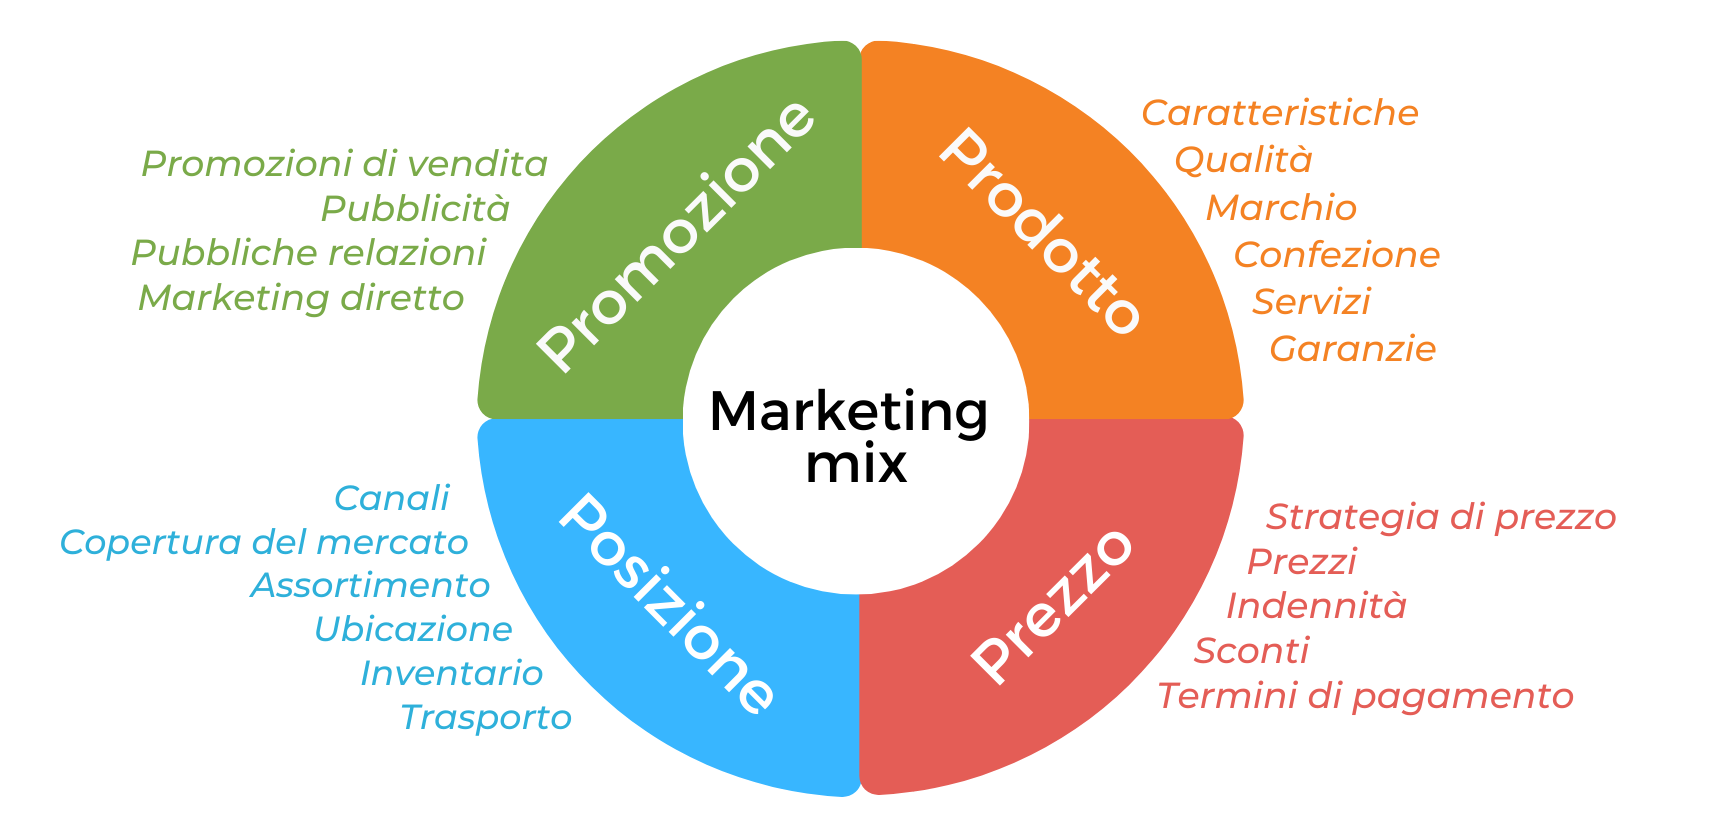
\includegraphics[width=0.7\linewidth]{resources/chapters/OrganizzazioneAziendale/images/pppp.png}
	\centering
	\caption{Riassunto della teoria delle quattro "P"}
\end{figure}